\section{Architecture Design}
\label{Architecture Design}

We followed Attribute-Driven Design (ADD)~\cite{clements2002documenting} to carry out the systematic creation of the architecture for our solution  based on the following key architectural drivers which include functional and Quality Attribute (QA) requirements:

\begin{enumerate}
    \item \textbf{Primary functional requirement}: the ability to generate code automatically from a visual design, which should accurately represent the intended behaviour.
    \item \textbf{QA1: Usability:} the solution should be as easy to use as possible.
    \item \textbf{QA2: Interoperability:} The solution should support the modelling of any correct design, which should be able to control a dynamic set of sensor and actuator devices.
   \item \textbf{QA3: Modularity:} The process of converting designs into code should be as modular as possible, so that we can use different transformation types to generate a variety of code in the future.
\end{enumerate}

The architectural drivers are used as the inputs to the architecture design process. This process involves several steps including the identification of architectural patterns and tactics, and documenting is using appropriate views. For our solution, the primary functional and quality attribute requirements are covered by two views: the logical view and the process view. These are described in the following subsections. 


\subsection{Logical view}

The logical view of our solution is presented as a class diagram in Fig.~\ref{fig:class}.
The logical view shows how a code base is structured to satisfy important architectural drivers.
It depicts how the functional requirements are achieved using successive model-to-model transformations of a given Activity Diagram Model into Java code.
These transformations are described in more detail in the next section.
The design of the Automatic Translation Tool is emphasized with the support of associations and compositions, which show how the primary functional requirement, as well as the desired quality of modularity.

\begin{figure}[!ht]
	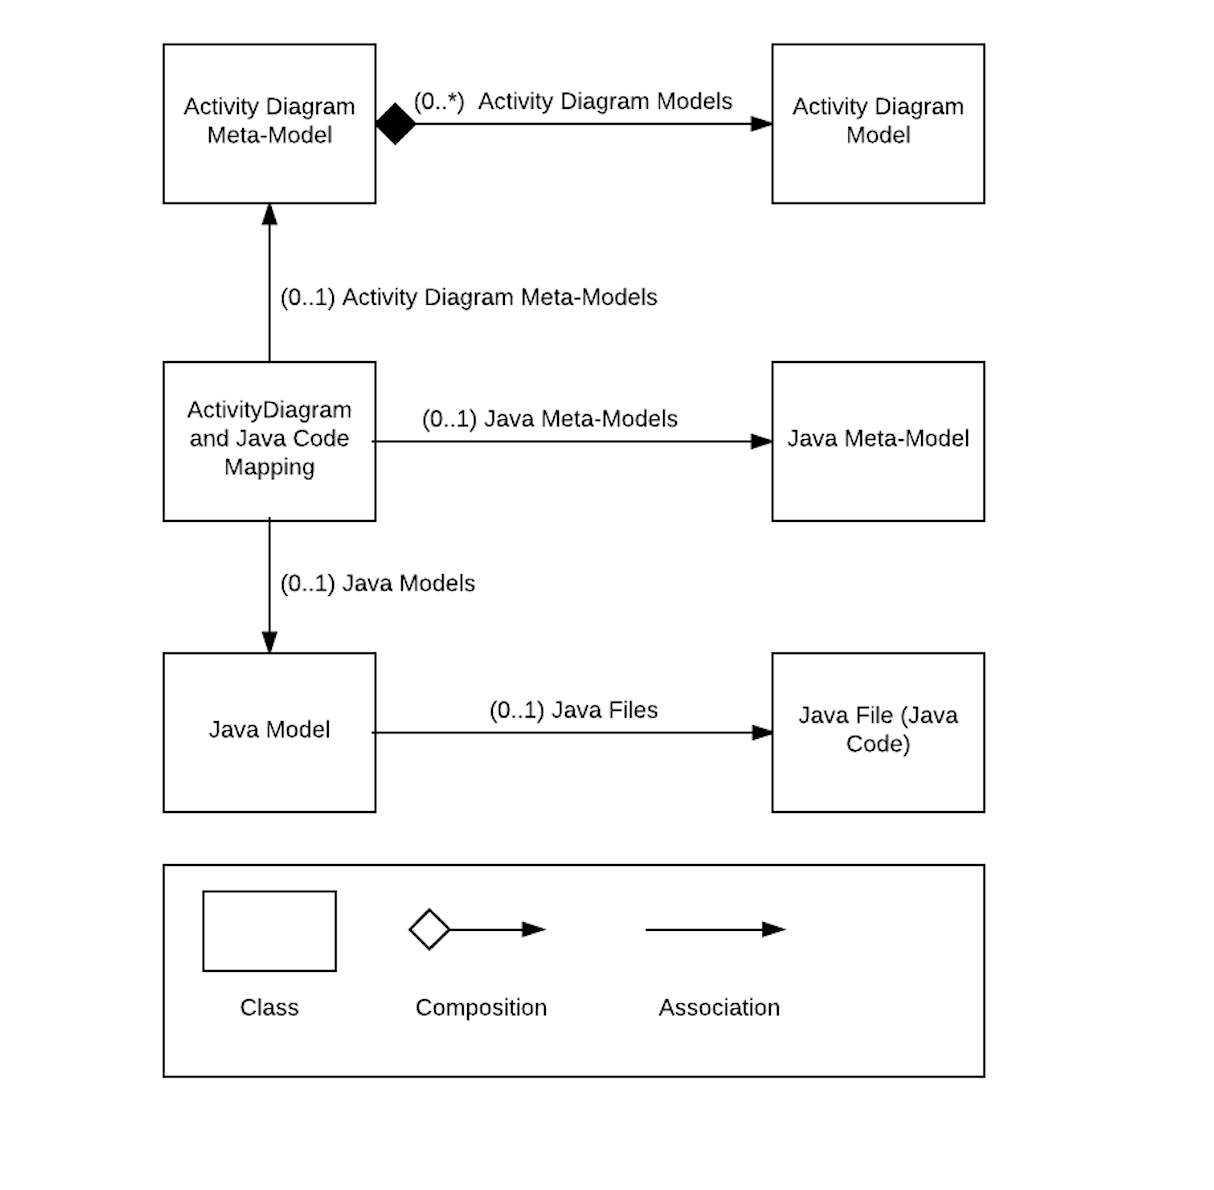
\includegraphics[width=\textwidth]{figs/Logical_View}
	\caption{UML Class Diagram: Automatic Translation Tool}
	\label{fig:class}
\end{figure}





\subsection{Process view}
The process view shows the dynamic aspects of the system and details the system processes and how the communication between various elements and entities are carried out when the system is operationalized~\cite{kruchten19954+}. The Activity Diagram shown in Fig.~\ref{figure:process} depicts the overall workflow of the tool's usage and ability to generate code in possibly different formats. The process view contributes to the key quality attributes of usability and interoperability.  

\begin{figure}[!h]
	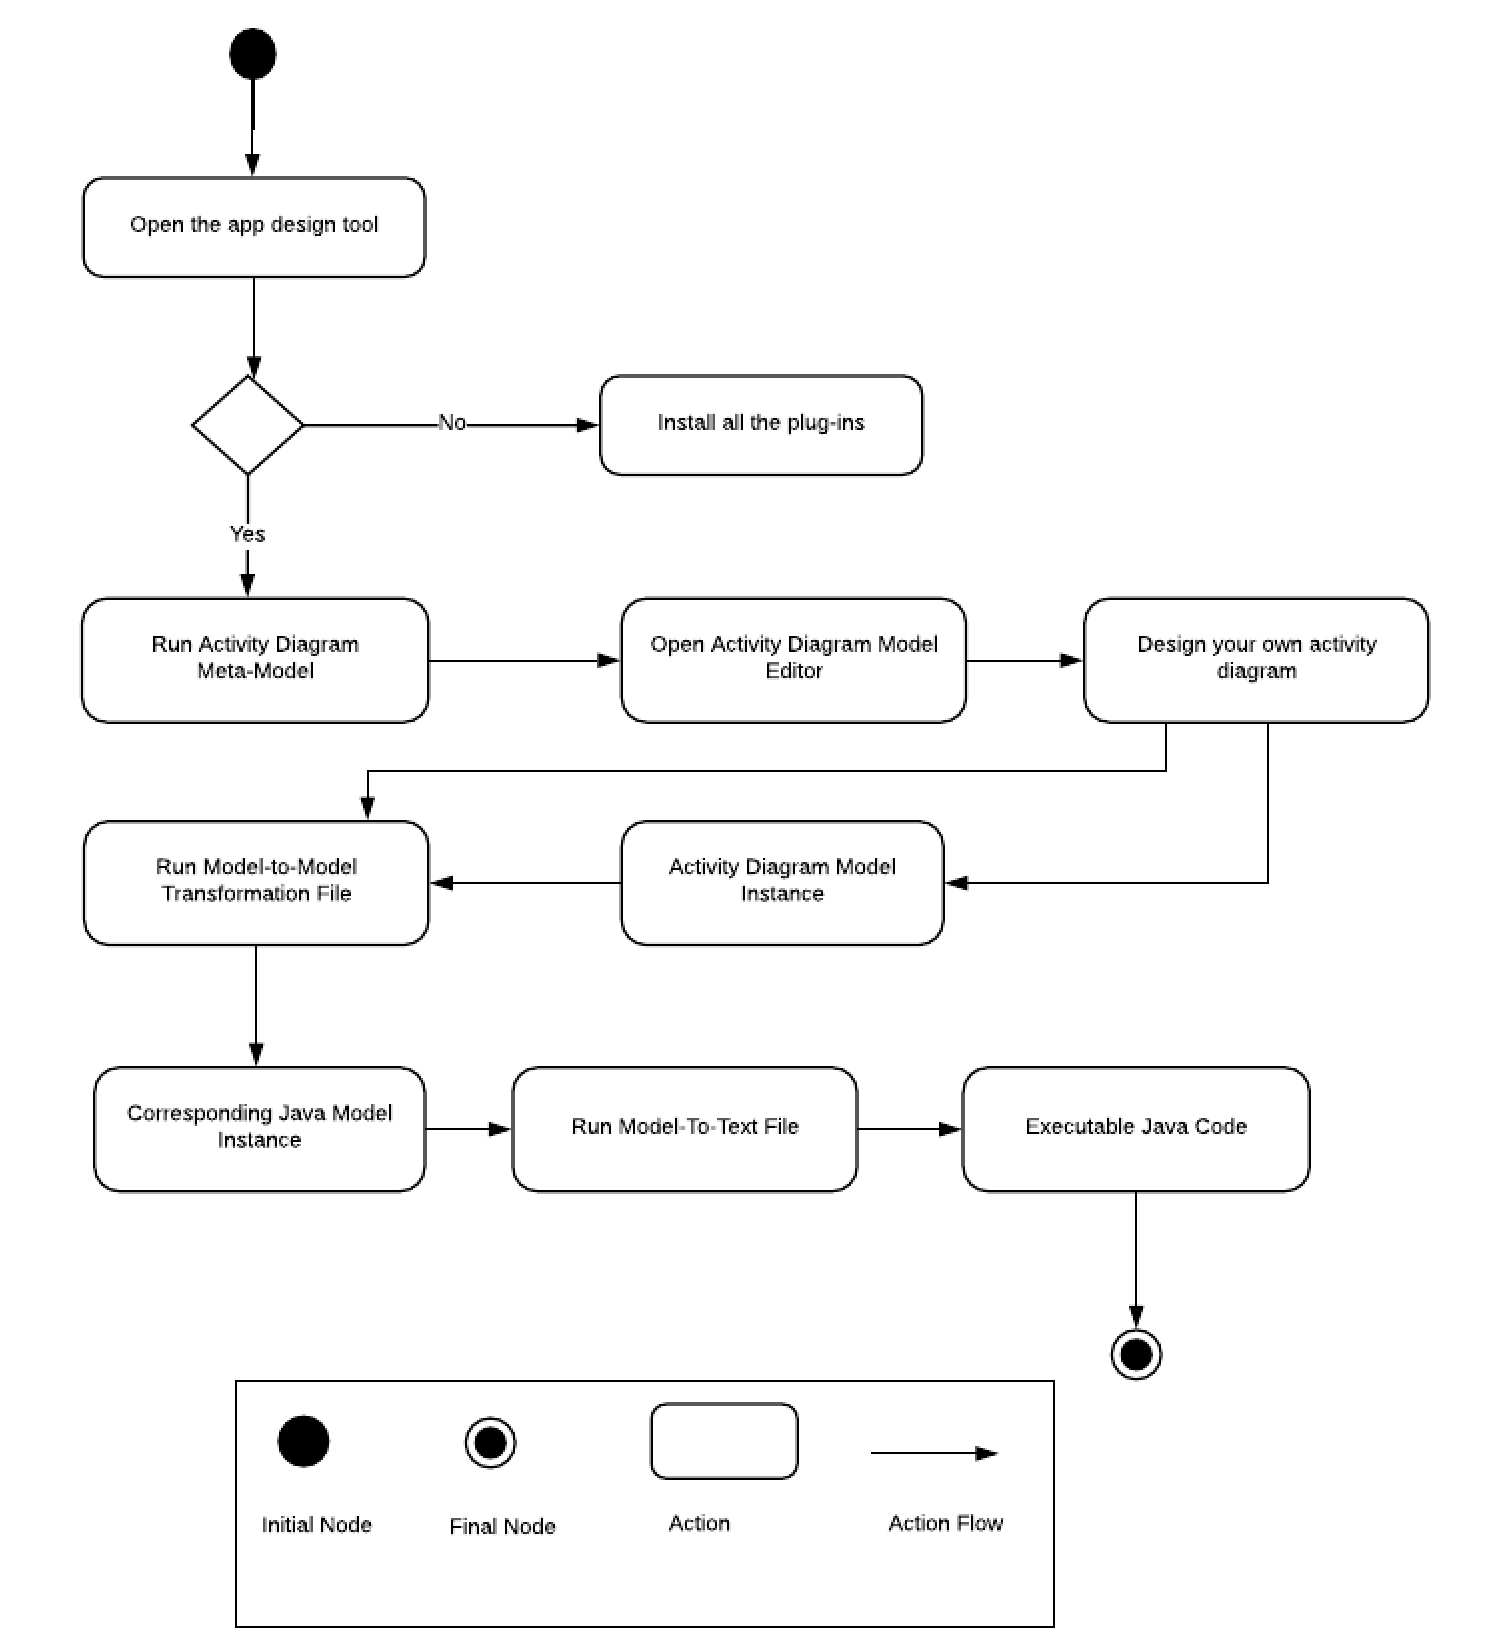
\includegraphics[width=\textwidth]{figs/ProcessView} 
	\caption{Process View}
	\label{figure:process}
\end{figure}



